\section{Hash, timestamping i blockchain}
\label{arquitectura:hash_timestamping}
%\textbf{Oscar}: \textit{Com es fa el hash i timestamping Introdueix l'esquema de CA i Blockchain}
%Una de les parts mes importants del sistema, per no dir la més important, és la capacitat d'assegurar el no repudi dels documents signats.\\
%\newline Aquesta capacitat de no repudi dels documents, s'aconsegueix mitjançant segellat de temps per una \textit{Timestamp Authorities} i publicant a la \textit{Blockchain} de \textit{Bitcoin}.\\
%\newline Per tant, un cop efectuada la signatura del document mitjançant el codi OTP, es genera el que s'anomena un comprovant de signatura. Aquest document, especifica que un usuari \textit{U}, en un moment determinat \textit{T}, ha signat amb un codi OTP \textit{O} un document amb empremta digital (hash) \textit{H}.\\
%\newline El \textit{hash} que es publicarà a la \textit{blockchain} o al que se li aplicarà el segellat de temps, és el del comprovant de signatura de creat anteriorment.
%\begin{figure}[h]
%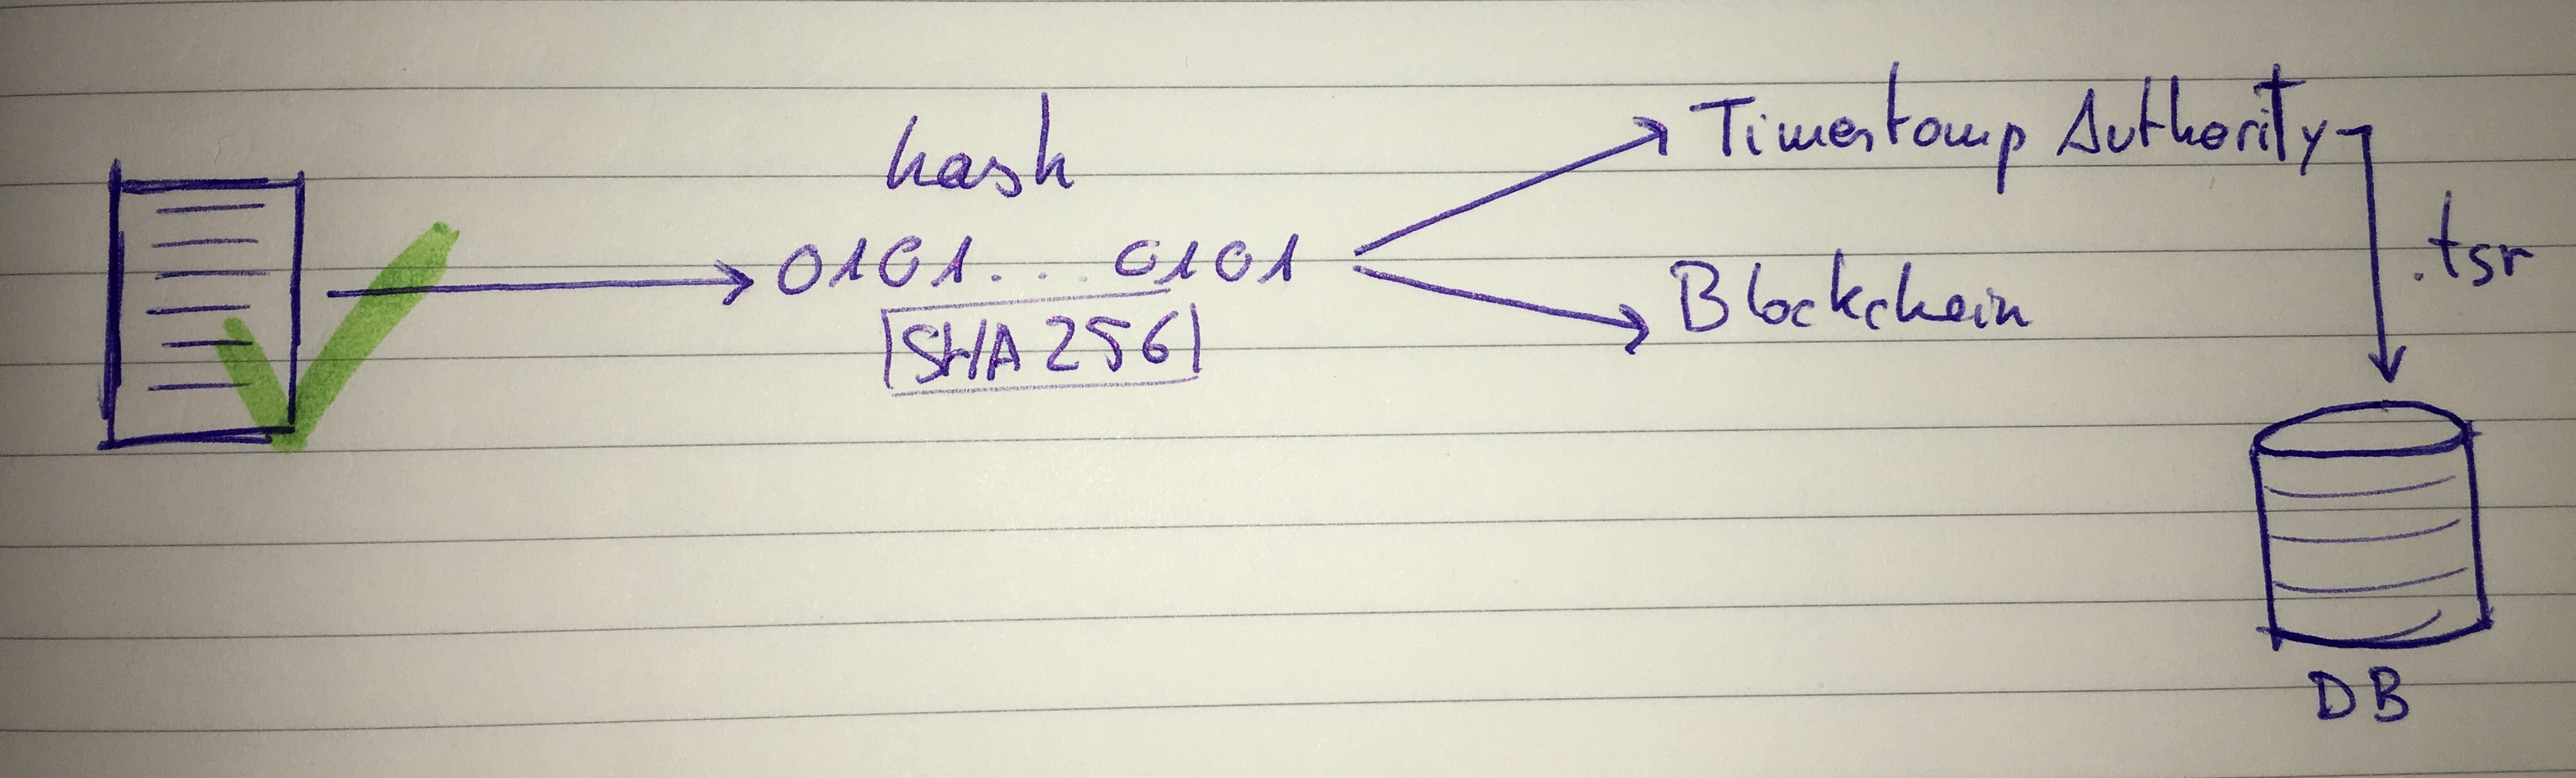
\includegraphics[scale=0.1]{sections/arquitectura/hash_timstamp_workflow.jpg}
%\centering
%\caption{Generació i certificació de documents}
%\label{fig:hash_timestamping_workflow}
%\end{figure}
%\newline A la figura anterior, es mostra el flux d'esdeveniments desencadenat per la signatura del consentiment informat.\\
%El \textit{hash} emprat, es calcula amb l'algorisme SHA256 i la funció de hash del propi llenguatge, a partir del contingut del document.\\
%\newline Seguint l'estructura de codi del projecte, ambdues funcionalitats (timestamping i blockchain) han estat encapsulades en serveis independents, per tal de que si en un moment moment donat es decideix canviar de tecnologia o de proveïdor de servei, per a la plataforma aquest canvi sigui totalment transparent.
%\clearpage
%\subsection{FreeTSA i timestamping}
\label{arquitectura:timestamping}
%Entrant més a baix nivell, d'acord amb l'standard definit a l'RFC3161\footnote{https://tools.ietf.org/html/rfc3161} el que s'anomena \textit{trusted timestamp} és un \textit{timestamp} emès per una  TSA\footnote{\textbf{T}ime \textbf{S}tamp \textbf{A}uthority} que es fa servir per a provar l'existència d'un cert contingut en un moment determinat.\\
%\newline A la figura següent (Figura \ref{fig:trusted_timestamping}) es pot veure el funcionament del procés de segellat de temps:
%\begin{figure}[h]
%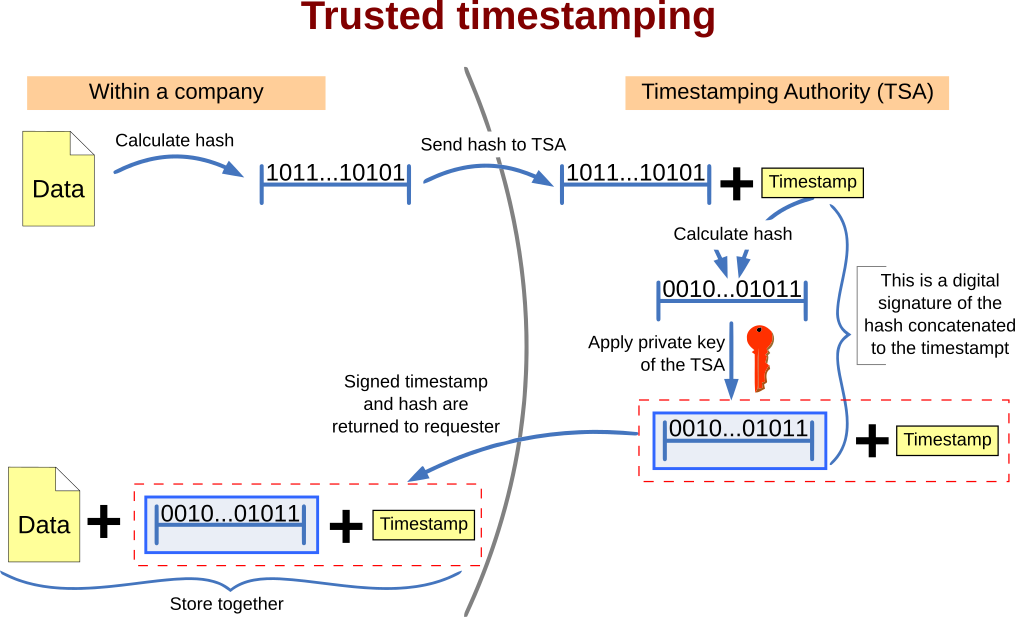
\includegraphics[scale=0.5]{sections/arquitectura/trusted_timestamping.png}
%\centering
%\caption{Generació i certificació de documents}
%\label{fig:trusted_timestamping}
%\end{figure}
%\newline A la figura anterior, es pot apreciar el funcionament del servei de segellat de temps de FreeTSA\footnote{https://freetsa.org/index_en.php} (entitat certificadora que es fa servir pel projecte).
%\newline En el cas concret del projecte, l'entitat que juga el rol de \textit{TSA}, és \textit{FreeTSA}\footnote{https://freetsa.org/index_en.php}.\\
%Com la gran majoria de serveis, ofereix una API (en aquest cas oberta) per a que els desenvolupadors puguin fer ús de les funcionalitats implementades.\\
%El funcionament del servei és ben senzill, primerament s'ha de generar un fitxer .tsq (\textit{time stamp query}) amb el contingut sobre el qual volem realitzar el segellat de temps. Aqesut fitxer, l'enviarem via HTTP/Post al servei de FreeTSA que respondrà amb un fitxer .tsr (\textit{time stamp request}).\\
%\newline Aquest fitxer .tsq, juntament amb els fitxers .pem i .tsc (donats pel mateix servei) ens serviràn posteriorment per validar el \textit{hash} dels documents.\\ És de vital importància el desar aquest fitxer .tsc, ja que és clau en el cas de necessitar defensar la integritat del comprovant de signatura mitjançant el segellat de temps.

Alternativament a l'ús de \textit{blockchain}, com a mesura de certificació addicional i per a donar més confiança, s'ha optat per donar al sistema un tercer cas d'ús.\\
\newline Tornant a la Figura \ref{fig:hash_timestamping_usecase}, al llarg d'aquesta secció es parlarà sobre el tercer i últim cas d'us, anomenat ``segellat de temps amb el hash''.\\
\newline Per aquest cas d'ús, es busca donar la confiança suficient a aquells que no vegin amb bons ulls l'ús de \textit{blockchain} com a mètode per a certificar l'existència d'un document en un instant de temps determinat.\\
Alhora, com s'ha dot anteriorment, suposa un extra que sempre és benvingut.\\
\newline Per aquesta ocasió, l'estructura i funcionament és molt similar al que s'ha vist la secció vista anteriorment (\ref{arquitectura:blockchain}). Dos serveis, un pertanyent a l'aplicació, amb l'objectiu d'encapsular i donar accés, i l'altre, un servei extern de tercers que ofereix funcions de segellat de temps.
\newline L'ús de serveis externs obliga a l'ús d'adaptadors que facin la funció d'enllaç entre l'aplicació desenvolupada per aquest projecte, i el servei extern.
% que ens permet realitzar el segellat de temps sobre el contingut d'un fitxer. Per a realitzar el segellat de temps, farem servir el \textit{hash} sobre el contingut d'aquest fitxer.


%\clearpage
%\subsection{OriginStamp i Blockchain}
\label{arquitectura:blockchain}
%With the advent of cryptocurrencies like Bitcoin, it has become possible to securely timestamp information in a decentralized and tamper-proof manner. Digital data can be hashed and the hash can be incorporated into a transaction stored in the blockchain, which serves as a secure proof of the exact time at which that data existed[2]. The proof is due to a tremendous amount of computational effort performed after the hash was submitted to the blockchain. Tampering with the timestamp would also lead to breaking the integrity of the entire digital currency, and this would result in the digital currency devaluing to zero[3].
%The decentralized timestamping approach using the Blockchain has also found applications in other areas, such as in dashboard cameras, to secure the integrity of video files at the time of their recording,[4] or to prove priority for creative content and ideas shared on social media platforms
Amb l'avanç de les anomenades criptomonedes (\textit{criptocurrencies} en anglès) com \textit{Bitcoin}, esdevé possible la creació de segells de temps d'una forma segura, descentralitzada i no modificable.\\
%\newline Així doncs, el \textit{hash} dels documents es poden incorporar a les transaccions i aquestes ser emmagatzemades a la \textit{blockchain}, que serveix com a prova de que en un instant determinat la informació a partir de la qual s'ha generat el \textit{hash}, existia.\\
%\newline El caràcter distribuït de la \textit{blockchain}, otorga irrefutabilitat a la prova d'existència, ja que ràpidament quedarà replicada als diferents nodes, aconseguint que la modificaició d'aquesta, sigui computacionalemnt impossible.\\
%\newline Així doncs serveis com \textit{OriginStamp}\footnote{https://app.originstamp.org/home} ofereixen la possibilitat de fer servir \textit{blockchain} per a certificar informació, en el context del TFG, el contingut dels comprovants de signatura generats.
%\begin{figure}[h]
%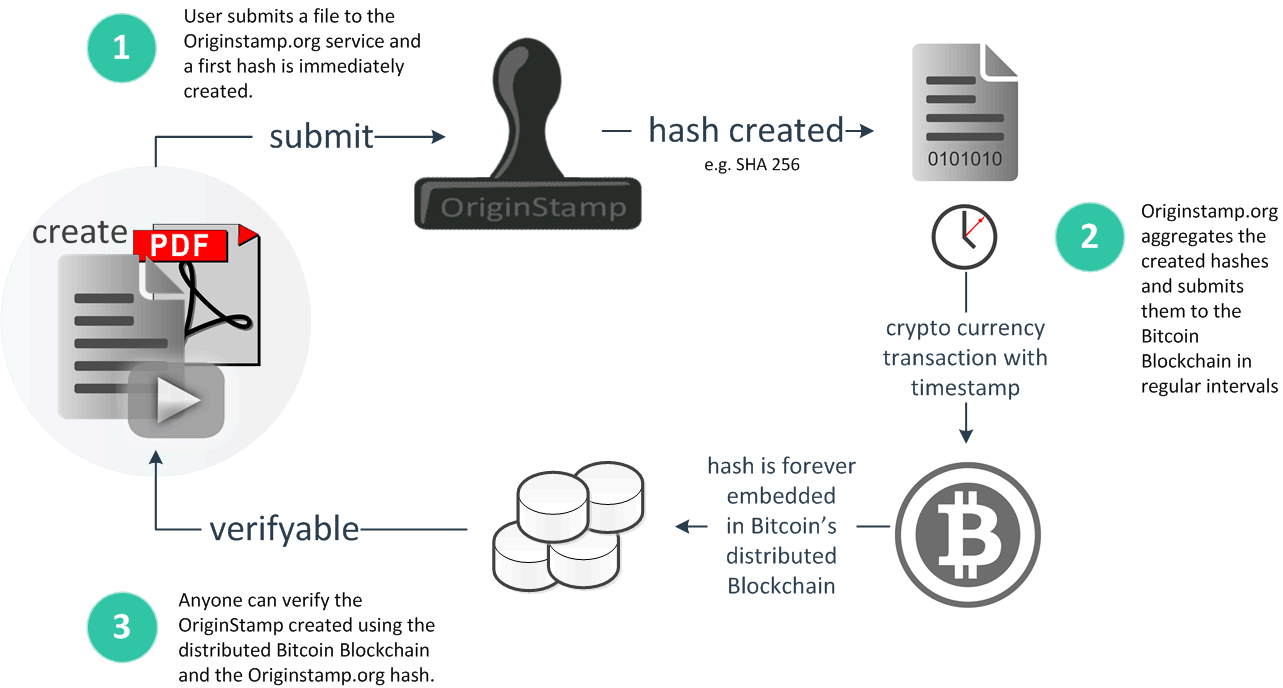
\includegraphics[scale=0.6]{sections/arquitectura/originStamp_workflow.png}
%\centering
%\caption{Funcionament d'OriginStamp}
%\label{fig:originstamp_workflow}
%\end{figure}
%\newline La Figura \ref{fig:originstamp_workflow} mostra el funcionament del servei \textit{OriginStamp}.\\
%Després de l'obtenció de la corresponent \textit{APIKey} per a poder realitzar operacions, manca encapsular les diferents funcionalitats en funcions php que facin les corrsponents crides a la API d'\textit{OriginStamp}.
\newline En el cas d'aquest TFG la creació d'un segell de temps és indispensable per a poder assolir l'objectiu final satisfactòriament.\\
\newline Al llarg d'aquesta secció es donaran detalls sobre els segon dels casos d'ús que es mostren a la Figura \ref{fig:hash_timestamping_usecase}, en concret al cas d'ús ``publicar hash a la blockchain''.\\
\newline De la mateixa manera que el component descrit a la secció \ref{arquitectura:generacio_documents}, aquest cas d'ús es composa de dos parts:
\begin{itemize}
    \item Un dels serveis del \textit{backend} desenvolupat, específicament per encapsular aquest cas d'ús i poder-lo fer servir des de qualsevol punt del projecte.
    Aquest servei respón a la necessitat d'un adaptador per a que el \textit{backend} es pugui comunicar amb el servei extern
    \item I per l'altre, el servei extern que permet publicar el \textit{hash} a la blockchain de bitcoin.\\
    Aquest servei extern, està dissenyat com una API Rest
\end{itemize}
La comunicació entre ambdós components es realitza a través de crides \textit{HTTP/Get} i \textit{HTTP/Post}, definides a documentació del servei.


Després de la generació de documents, el pas següent resideix en la certificació del contingut d'aquests.\\
\newline Per a dur a terme aquesta tasca, i seguint amb l'arquitectura presentada anteriorment (\nameref{arquitectura:back_clean}), s'han separat els diferents casos d'ús en serveis independents.
\begin{figure}[h]
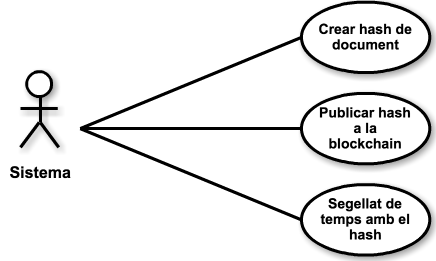
\includegraphics[scale=0.4]{sections/arquitectura/hashTimestamping_usecase.png}
\centering
\caption{Hash i timestamping - Cas d'ús}
\label{fig:hash_timestamping_usecase}
\end{figure}
\newline La Figura \ref{fig:hash_timestamping_usecase} ens mostra els diferents casos d'ús d'aquesta part del sistema d'emissió i validació.\\
%\begin{itemize}
%    \item El primer cas d'ús, referent a la creació del hash, serveix com a capa d'abstracció per a per a poder usar aquesta funcionalitat independentment des de qualsevol punt del projecte.\\ 
%    L'entrada ha de ser forçosament la ruta a un fitxer existent.\\
%    La sortida, és una cadena de caràcters basada en el contingut del fitxer d'entrada.
%    \item Aquest segon cas d'ús, publicació del hash a la \textit{blockchain}, fa referència a un primer i principal mètode de certificació de la signatura.
%    \item Finalment, aquest tercer cas d'ús, ús de segellat de temps, busca donar un grau més de seguretat al procés de signatura electrònica descrit anteriorment.
%\end{itemize}
%Al llarg de les pròximes seccions es tractarà amb més detall els casos d'ús que fan referència a la certificació del contingut dels documents.
%\clearpage
%\subsection{OriginStamp i Blockchain}
\label{arquitectura:blockchain}
%With the advent of cryptocurrencies like Bitcoin, it has become possible to securely timestamp information in a decentralized and tamper-proof manner. Digital data can be hashed and the hash can be incorporated into a transaction stored in the blockchain, which serves as a secure proof of the exact time at which that data existed[2]. The proof is due to a tremendous amount of computational effort performed after the hash was submitted to the blockchain. Tampering with the timestamp would also lead to breaking the integrity of the entire digital currency, and this would result in the digital currency devaluing to zero[3].
%The decentralized timestamping approach using the Blockchain has also found applications in other areas, such as in dashboard cameras, to secure the integrity of video files at the time of their recording,[4] or to prove priority for creative content and ideas shared on social media platforms
Amb l'avanç de les anomenades criptomonedes (\textit{criptocurrencies} en anglès) com \textit{Bitcoin}, esdevé possible la creació de segells de temps d'una forma segura, descentralitzada i no modificable.\\
%\newline Així doncs, el \textit{hash} dels documents es poden incorporar a les transaccions i aquestes ser emmagatzemades a la \textit{blockchain}, que serveix com a prova de que en un instant determinat la informació a partir de la qual s'ha generat el \textit{hash}, existia.\\
%\newline El caràcter distribuït de la \textit{blockchain}, otorga irrefutabilitat a la prova d'existència, ja que ràpidament quedarà replicada als diferents nodes, aconseguint que la modificaició d'aquesta, sigui computacionalemnt impossible.\\
%\newline Així doncs serveis com \textit{OriginStamp}\footnote{https://app.originstamp.org/home} ofereixen la possibilitat de fer servir \textit{blockchain} per a certificar informació, en el context del TFG, el contingut dels comprovants de signatura generats.
%\begin{figure}[h]
%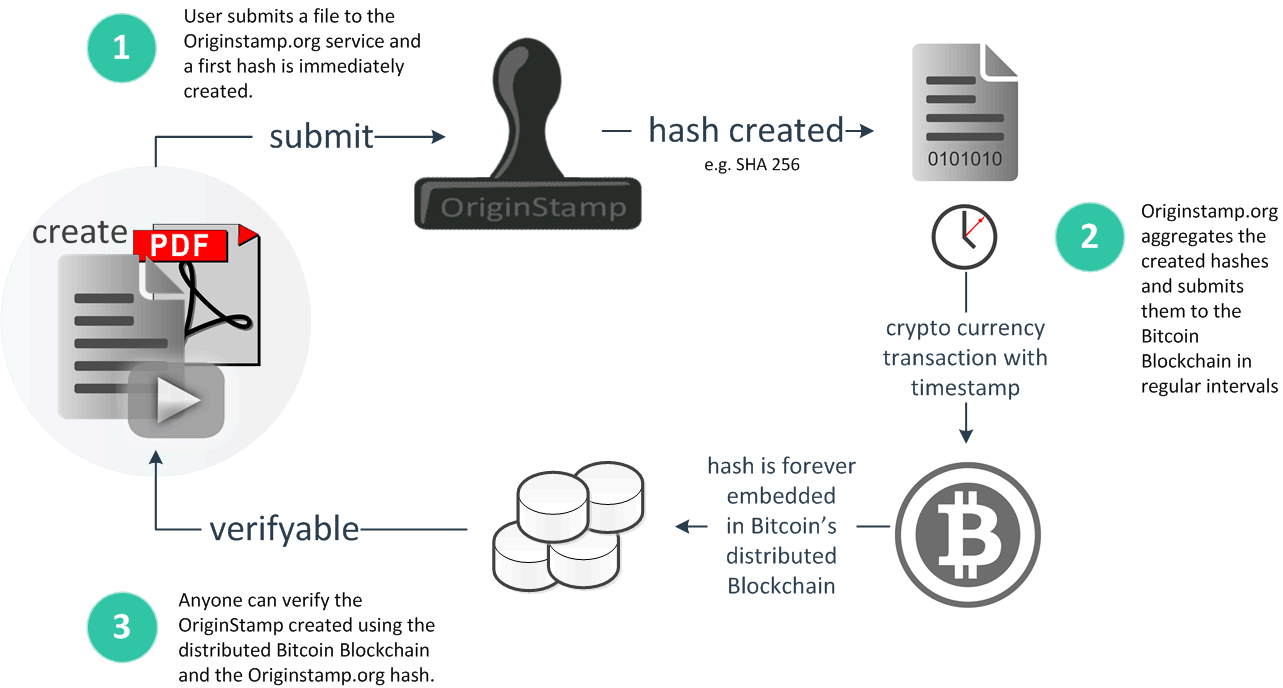
\includegraphics[scale=0.6]{sections/arquitectura/originStamp_workflow.png}
%\centering
%\caption{Funcionament d'OriginStamp}
%\label{fig:originstamp_workflow}
%\end{figure}
%\newline La Figura \ref{fig:originstamp_workflow} mostra el funcionament del servei \textit{OriginStamp}.\\
%Després de l'obtenció de la corresponent \textit{APIKey} per a poder realitzar operacions, manca encapsular les diferents funcionalitats en funcions php que facin les corrsponents crides a la API d'\textit{OriginStamp}.
\newline En el cas d'aquest TFG la creació d'un segell de temps és indispensable per a poder assolir l'objectiu final satisfactòriament.\\
\newline Al llarg d'aquesta secció es donaran detalls sobre els segon dels casos d'ús que es mostren a la Figura \ref{fig:hash_timestamping_usecase}, en concret al cas d'ús ``publicar hash a la blockchain''.\\
\newline De la mateixa manera que el component descrit a la secció \ref{arquitectura:generacio_documents}, aquest cas d'ús es composa de dos parts:
\begin{itemize}
    \item Un dels serveis del \textit{backend} desenvolupat, específicament per encapsular aquest cas d'ús i poder-lo fer servir des de qualsevol punt del projecte.
    Aquest servei respón a la necessitat d'un adaptador per a que el \textit{backend} es pugui comunicar amb el servei extern
    \item I per l'altre, el servei extern que permet publicar el \textit{hash} a la blockchain de bitcoin.\\
    Aquest servei extern, està dissenyat com una API Rest
\end{itemize}
La comunicació entre ambdós components es realitza a través de crides \textit{HTTP/Get} i \textit{HTTP/Post}, definides a documentació del servei.


%\subsection{FreeTSA i timestamping}
\label{arquitectura:timestamping}
%Entrant més a baix nivell, d'acord amb l'standard definit a l'RFC3161\footnote{https://tools.ietf.org/html/rfc3161} el que s'anomena \textit{trusted timestamp} és un \textit{timestamp} emès per una  TSA\footnote{\textbf{T}ime \textbf{S}tamp \textbf{A}uthority} que es fa servir per a provar l'existència d'un cert contingut en un moment determinat.\\
%\newline A la figura següent (Figura \ref{fig:trusted_timestamping}) es pot veure el funcionament del procés de segellat de temps:
%\begin{figure}[h]
%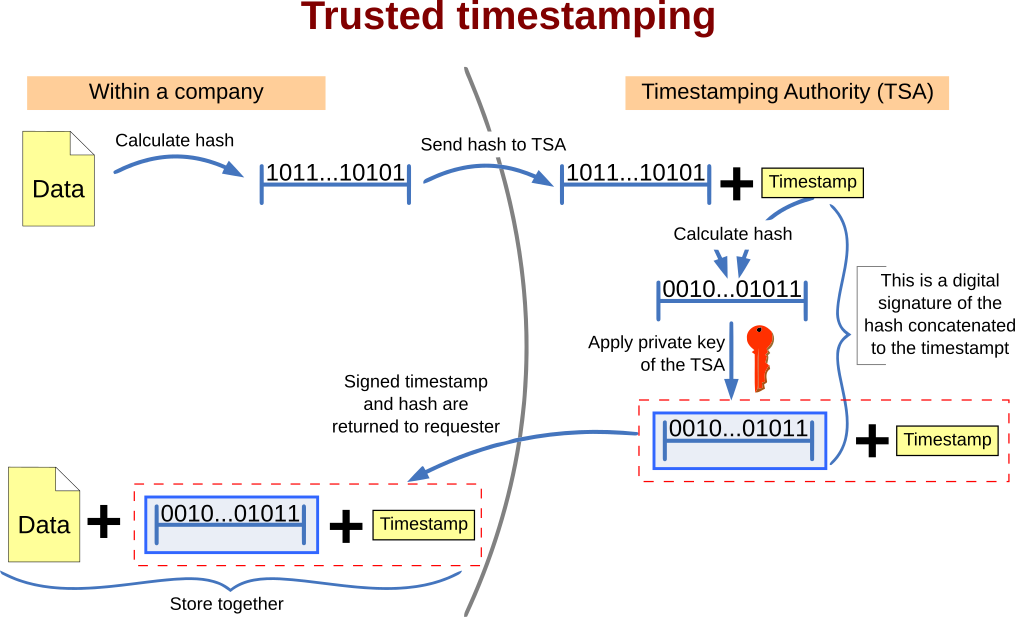
\includegraphics[scale=0.5]{sections/arquitectura/trusted_timestamping.png}
%\centering
%\caption{Generació i certificació de documents}
%\label{fig:trusted_timestamping}
%\end{figure}
%\newline A la figura anterior, es pot apreciar el funcionament del servei de segellat de temps de FreeTSA\footnote{https://freetsa.org/index_en.php} (entitat certificadora que es fa servir pel projecte).
%\newline En el cas concret del projecte, l'entitat que juga el rol de \textit{TSA}, és \textit{FreeTSA}\footnote{https://freetsa.org/index_en.php}.\\
%Com la gran majoria de serveis, ofereix una API (en aquest cas oberta) per a que els desenvolupadors puguin fer ús de les funcionalitats implementades.\\
%El funcionament del servei és ben senzill, primerament s'ha de generar un fitxer .tsq (\textit{time stamp query}) amb el contingut sobre el qual volem realitzar el segellat de temps. Aqesut fitxer, l'enviarem via HTTP/Post al servei de FreeTSA que respondrà amb un fitxer .tsr (\textit{time stamp request}).\\
%\newline Aquest fitxer .tsq, juntament amb els fitxers .pem i .tsc (donats pel mateix servei) ens serviràn posteriorment per validar el \textit{hash} dels documents.\\ És de vital importància el desar aquest fitxer .tsc, ja que és clau en el cas de necessitar defensar la integritat del comprovant de signatura mitjançant el segellat de temps.

Alternativament a l'ús de \textit{blockchain}, com a mesura de certificació addicional i per a donar més confiança, s'ha optat per donar al sistema un tercer cas d'ús.\\
\newline Tornant a la Figura \ref{fig:hash_timestamping_usecase}, al llarg d'aquesta secció es parlarà sobre el tercer i últim cas d'us, anomenat ``segellat de temps amb el hash''.\\
\newline Per aquest cas d'ús, es busca donar la confiança suficient a aquells que no vegin amb bons ulls l'ús de \textit{blockchain} com a mètode per a certificar l'existència d'un document en un instant de temps determinat.\\
Alhora, com s'ha dot anteriorment, suposa un extra que sempre és benvingut.\\
\newline Per aquesta ocasió, l'estructura i funcionament és molt similar al que s'ha vist la secció vista anteriorment (\ref{arquitectura:blockchain}). Dos serveis, un pertanyent a l'aplicació, amb l'objectiu d'encapsular i donar accés, i l'altre, un servei extern de tercers que ofereix funcions de segellat de temps.
\newline L'ús de serveis externs obliga a l'ús d'adaptadors que facin la funció d'enllaç entre l'aplicació desenvolupada per aquest projecte, i el servei extern.
% que ens permet realitzar el segellat de temps sobre el contingut d'un fitxer. Per a realitzar el segellat de temps, farem servir el \textit{hash} sobre el contingut d'aquest fitxer.


\subsubsection{Crear hash de document}
%Serveix com a capa d'abstracció per a per a poder usar aquesta funcionalitat independentment des de qualsevol punt del projecte.\\ 
%L'entrada ha de ser forçosament la ruta a un fitxer existent.\\
%La sortida, és una cadena de caràcters basada en el contingut del fitxer d'entrada.
Un cop s'ha signat el consentiment informat i s'ha generat el comprovant de signatura, el sistema ha de calcular el hash del comprovant per tal de poder certificar-lo (casos d'ús següents).\\
\newline Seguint amb l'arquitectura vista al principi del capítol (\nameref{arquitectura:back_clean}), la fucionalitat s'encapsula en un servei per a poder fer-la servir en qualsevol punt mitjançant la injecció de dependències que proposen els principis \nameref{arquitectura:back_solid}.\\
\newline A la següent figura es pot veure el comportament del servei vers el sistema:
\begin{figure}[h]
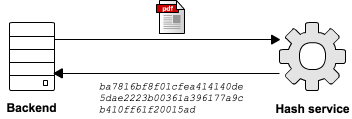
\includegraphics[scale=0.5]{sections/arquitectura/hashTimestamping_hashService.png}
\centering
\caption{Hash i timestamping - Hash service}
\label{fig:hash_timestamping_hashService}
\end{figure}
\newline Tal i com il·lustra la figura anterior, l'entrada del servei ha de ser un document, en el cas de la figura pdf, o en el seu defecte la ruta al fitxer.\\
Si la ruta/fitxer és correcte, el servei retorna hash.
\clearpage
%El sistema ha de ser capaç de crear un \textit{hash} a partir de documents existents.\\
%De la mateixa manera, 
\subsubsection{Publicar hash a la \textit{blockchain}}
De la mateixa manera que el component descrit a la secció \ref{arquitectura:generacio_documents}, aquest cas d'ús es composa de dos parts:
\begin{itemize}
    \item Un dels serveis del \textit{backend}, desenvolupat específicament per encapsular aquest cas d'ús i poder-lo fer servir des de qualsevol punt del projecte.
    Aquest servei respon a la necessitat d'un adaptador per a que el \textit{backend} es pugui comunicar amb el servei extern
    \item I per l'altra, el servei extern que permet publicar el \textit{hash} a la blockchain de bitcoin.\\
    Aquest servei extern, està dissenyat com una API Rest
\end{itemize}
La comunicació entre ambdós components es realitza a través de crides \textit{HTTP/Get} i \textit{HTTP/Post}, definides a documentació del servei.\\
\newline Amb una finalitat merament il·lustrativa, aquest cas d'ús respondria a una arquitectura similar a la que mostra la figura següent:
\begin{figure}[h]
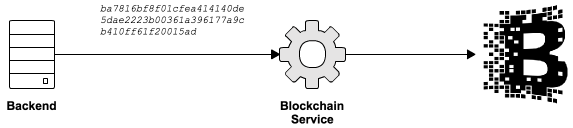
\includegraphics[scale=0.5]{sections/arquitectura/hashTimestamping_blockchainService.png}
\centering
\caption{Hash i timestamping - Blockchain service}
\label{fig:hash_timestamping_blockchainService}
\end{figure}
\subsubsection{Segellat de temps amb el hash}
Amb aquest cas d'ús, es busca donar la confiança suficient, a aquells que no vegin amb bons ulls, l'ús de \textit{blockchain} com a mètode per a certificar l'existència d'un document en un instant de temps determinat.\\
Tant mateix, com s'ha dit anteriorment, suposa un extra important en el moment de defensar la immutabilitat dels documents.\\
\newline Per aquesta ocasió, l'estructura i funcionament és molt similar al que s'ha vist en el cas d'ús anterior. Dos serveis, un pertanyent a l'aplicació, amb l'objectiu d'encapsular i donar accés des de qualsevol punt de la plataforma, i l'altre, un servei extern de tercers que ofereix funcions de segellat de temps.
%\newline L'ús de serveis externs obliga a l'ús d'adaptadors que facin la funció d'enllaç entre l'aplicació desenvolupada per aquest projecte, i el servei extern.